
\documentclass[11pt]{exam} % https://www.ctan.org/pkg/exam?lang=en

\usepackage[lmargin=1.in,rmargin=1.in,tmargin=1.in,bmargin=1in]{geometry}
\usepackage{setspace}
\usepackage[pdftex]{graphicx}
\usepackage{titling}
\usepackage[
	pdfauthor={Brian Weinstein},
	pdftitle={Homework 1},
	bookmarks=true,
	colorlinks=true,
	linkcolor=blue,
	urlcolor=blue,
	citecolor=blue,
	pdftex,
	linktocpage=true
	]{hyperref}
\usepackage[textsize=tiny]{todonotes}
\usepackage{float}
\setlength\parindent{0pt}
\usepackage{lipsum}


\qformat{\textbf{Problem \thequestion: \thequestiontitle}\quad \hfill}


\pagestyle{headandfoot}
\runningheadrule
\firstpageheader{}{}{}
\runningheader{\theauthor}{\thetitle}{\thedate}
\firstpagefooter{}{\thepage}{}
\runningfooter{}{\thepage}{}


\usepackage{xcolor}
\usepackage{adjustbox}
\usepackage{verbatim}
\definecolor{shadecolor}{rgb}{.9, .9, .9}

\newenvironment{code}%
   {\par\noindent\adjustbox{margin=1ex,bgcolor=shadecolor,margin=0ex \medskipamount}\bgroup\minipage\linewidth\verbatim}%
   {\endverbatim\endminipage\egroup}

\newenvironment{codeSmall}%
   {\par\noindent\adjustbox{margin=1ex,bgcolor=shadecolor,margin=0ex \medskipamount}\bgroup\minipage\linewidth\verbatim\footnotesize}%
   {\endverbatim\endminipage\egroup}

\newcommand{\ramsey}{\href{http://www.statisticalsleuth.com/}{Ramsey }}



\begin{document}


\title{STAT S4201 001, Homework 1}
\author{Brian Weinstein (bmw2148)}
\date{Feb 3, 2016}
\maketitle



\begin{questions}


\titledquestion{\ramsey 1.17}

See \texttt{hw01.R} for code.

The observed difference between sample averages is $15.333$, which, based on the 35 differences in the randomization distribution, corresponds to a two-sided p-value of $0.0867$.



\titledquestion{\ramsey 1.21} \todo{problem 2 (1.21)}

\begin{parts}

\part A Trial of Wound Irrigation in the Initial Management of Open Fracture Wounds

\begin{subparts}

\subpart Link: \href{http://www.nejm.org/doi/full/10.1056/NEJMoa1508502}{http://www.nejm.org/doi/full/10.1056/NEJMoa1508502}

\subpart Study design and conclusions:

asdfasdf

\subpart Categorize the study according to Display 1.5.

asdfasdf

\subpart Determine whether inferential statements are limited to or go beyond the scope allowed in Display 1.5.

asdfasdf

\end{subparts}






\part A Randomized, Controlled Trial of an Aerosolized Vaccine against Measles


\begin{subparts}

\subpart Link: \href{http://www.nejm.org/doi/full/10.1056/NEJMoa1407417}{http://www.nejm.org/doi/full/10.1056/NEJMoa1407417}

\subpart Study design and conclusions:

asdfasdf

\subpart Categorize the study according to Display 1.5.

asdfasdf

\subpart Determine whether inferential statements are limited to or go beyond the scope allowed in Display 1.5.

asdfasdf

\end{subparts}





\end{parts}




\titledquestion{\ramsey 1.25 (b)}

See Figure \ref{fig:3}.

\begin{figure}[h!]
	\centering
	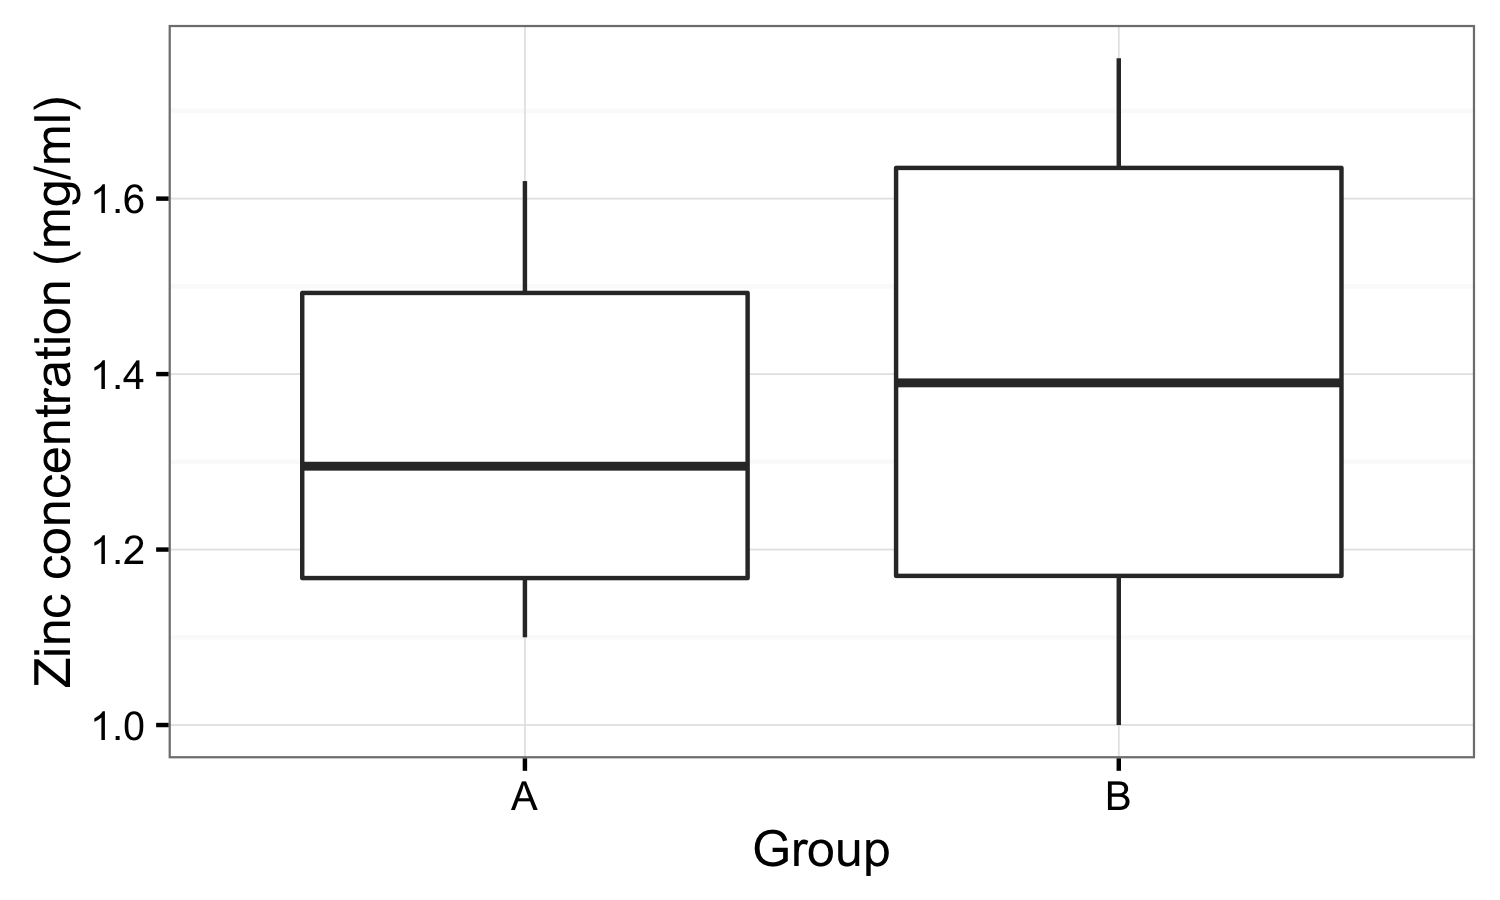
\includegraphics[width=5in]{3.png}
	\caption{Zinc concentrations (in mg/ml) in the blood for two groups of rats. Group A received a calcium supplement and Group B did not.}
	\label{fig:3}
\end{figure}




\titledquestion{Use the data from Problem 3 to answer the following questions.}

\begin{parts}

\part Set up the null and alternative hypotheses to address the research question described.

\begin{itemize}
\item Test statistic $t=\bar{A}-\bar{B}$, where $\bar{A}$ and $\bar{B}$ are the average Zinc concentrations in the rats of group A and B, respectively.
\item Null hypothesis: $t=0$
\item Alternative hypothesis: $t\neq0$
\end{itemize}


\part Use 1,000 simulations to perform a randomization test for testing the hypothesis in (a). What is your p-value?

The observed difference between sample averages is $-0.07755$, which, based on the 1,000 simulations in the randomization distribution, corresponds to a two-sided p-value of $0.261$.

\part Draw the reference distribution of your test statistic based on 1,000 simulations.

See Figure \ref{fig:4c}.

\begin{figure}[h!]
	\centering
	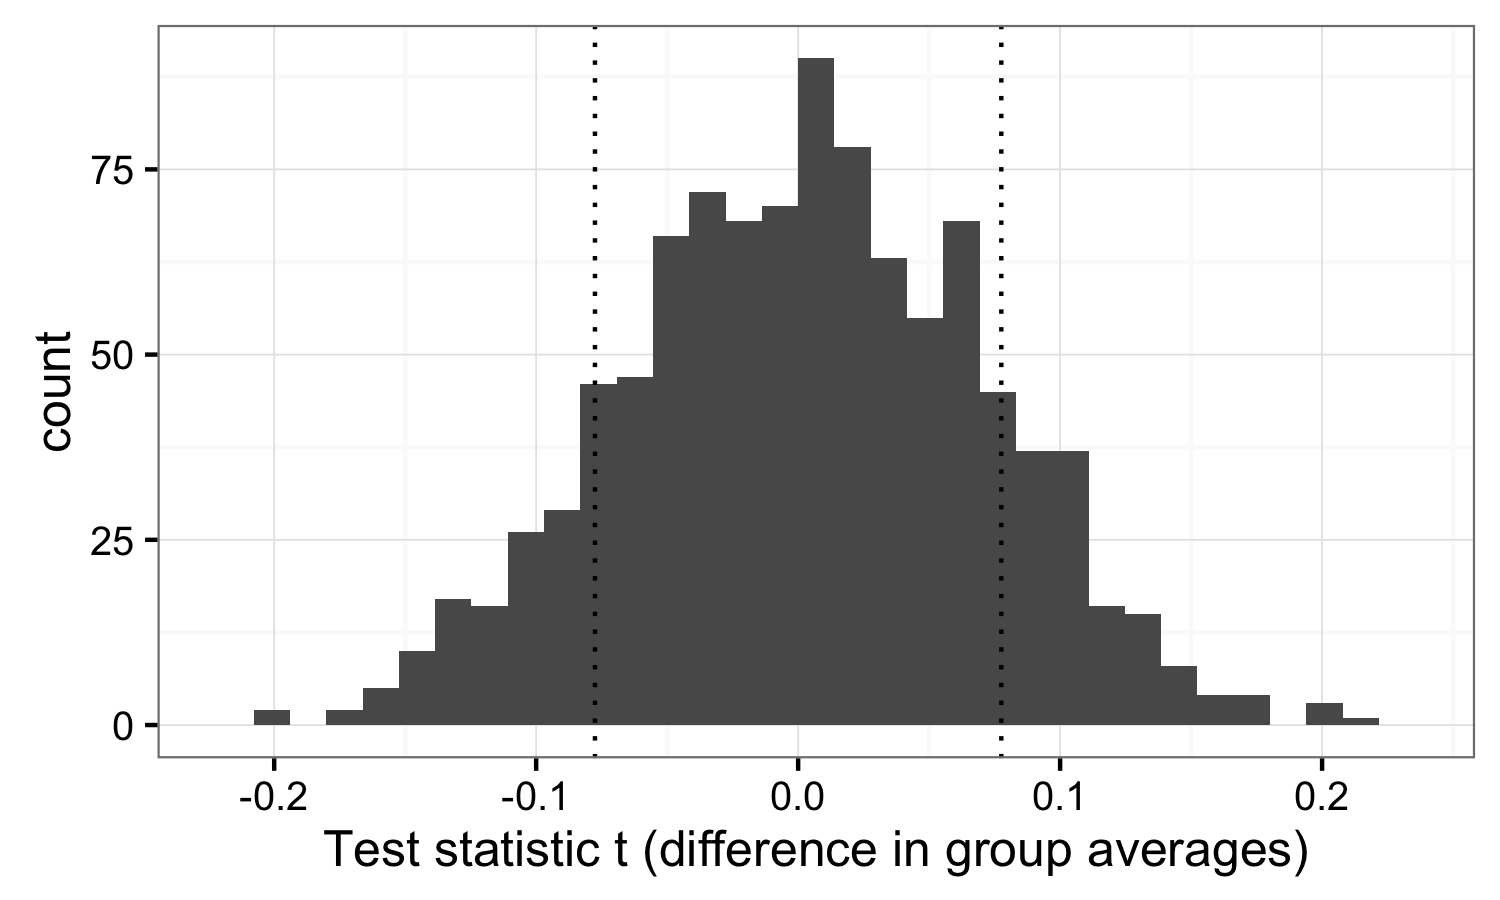
\includegraphics[width=5in]{4c.png}
	\caption{Reference distribution of $t$, based on 1,000 simulations.}
	\label{fig:4c}
\end{figure}


\part Write a brief summary of your findings and possible recommendations for the researchers.

\todo{problem 4d}




\end{parts}





\titledquestion{question name}

\begin{parts}



\part asdf asdf asdf
\begin{code}
> apply(rawData, 2, mean)
       x1        x2        x3        x4        x5 
 6.049104 -8.277221  4.665532  7.914270 62.138753 
\end{code}
 
\part asdfasdfasdf


\begin{subparts}

\subpart asdf asdf asdf asdf

\begin{codeSmall}
> apply(rawData, 1, mean)
  [1]  -0.1277116  20.8162864  -8.8984358  25.5999204  -9.7472153
  [6]  64.0626702  22.0392371  23.3914888  31.7598224 -13.8680290
...
 [91]   1.2105932  21.2145724  -8.4896595  19.0639963  20.9767512
 [96]   3.5962333  22.3461063   0.7145014   6.3080005  64.8829556
\end{codeSmall}

\end{subparts}
 
%\begin{figure}[H]
%	\centering
%	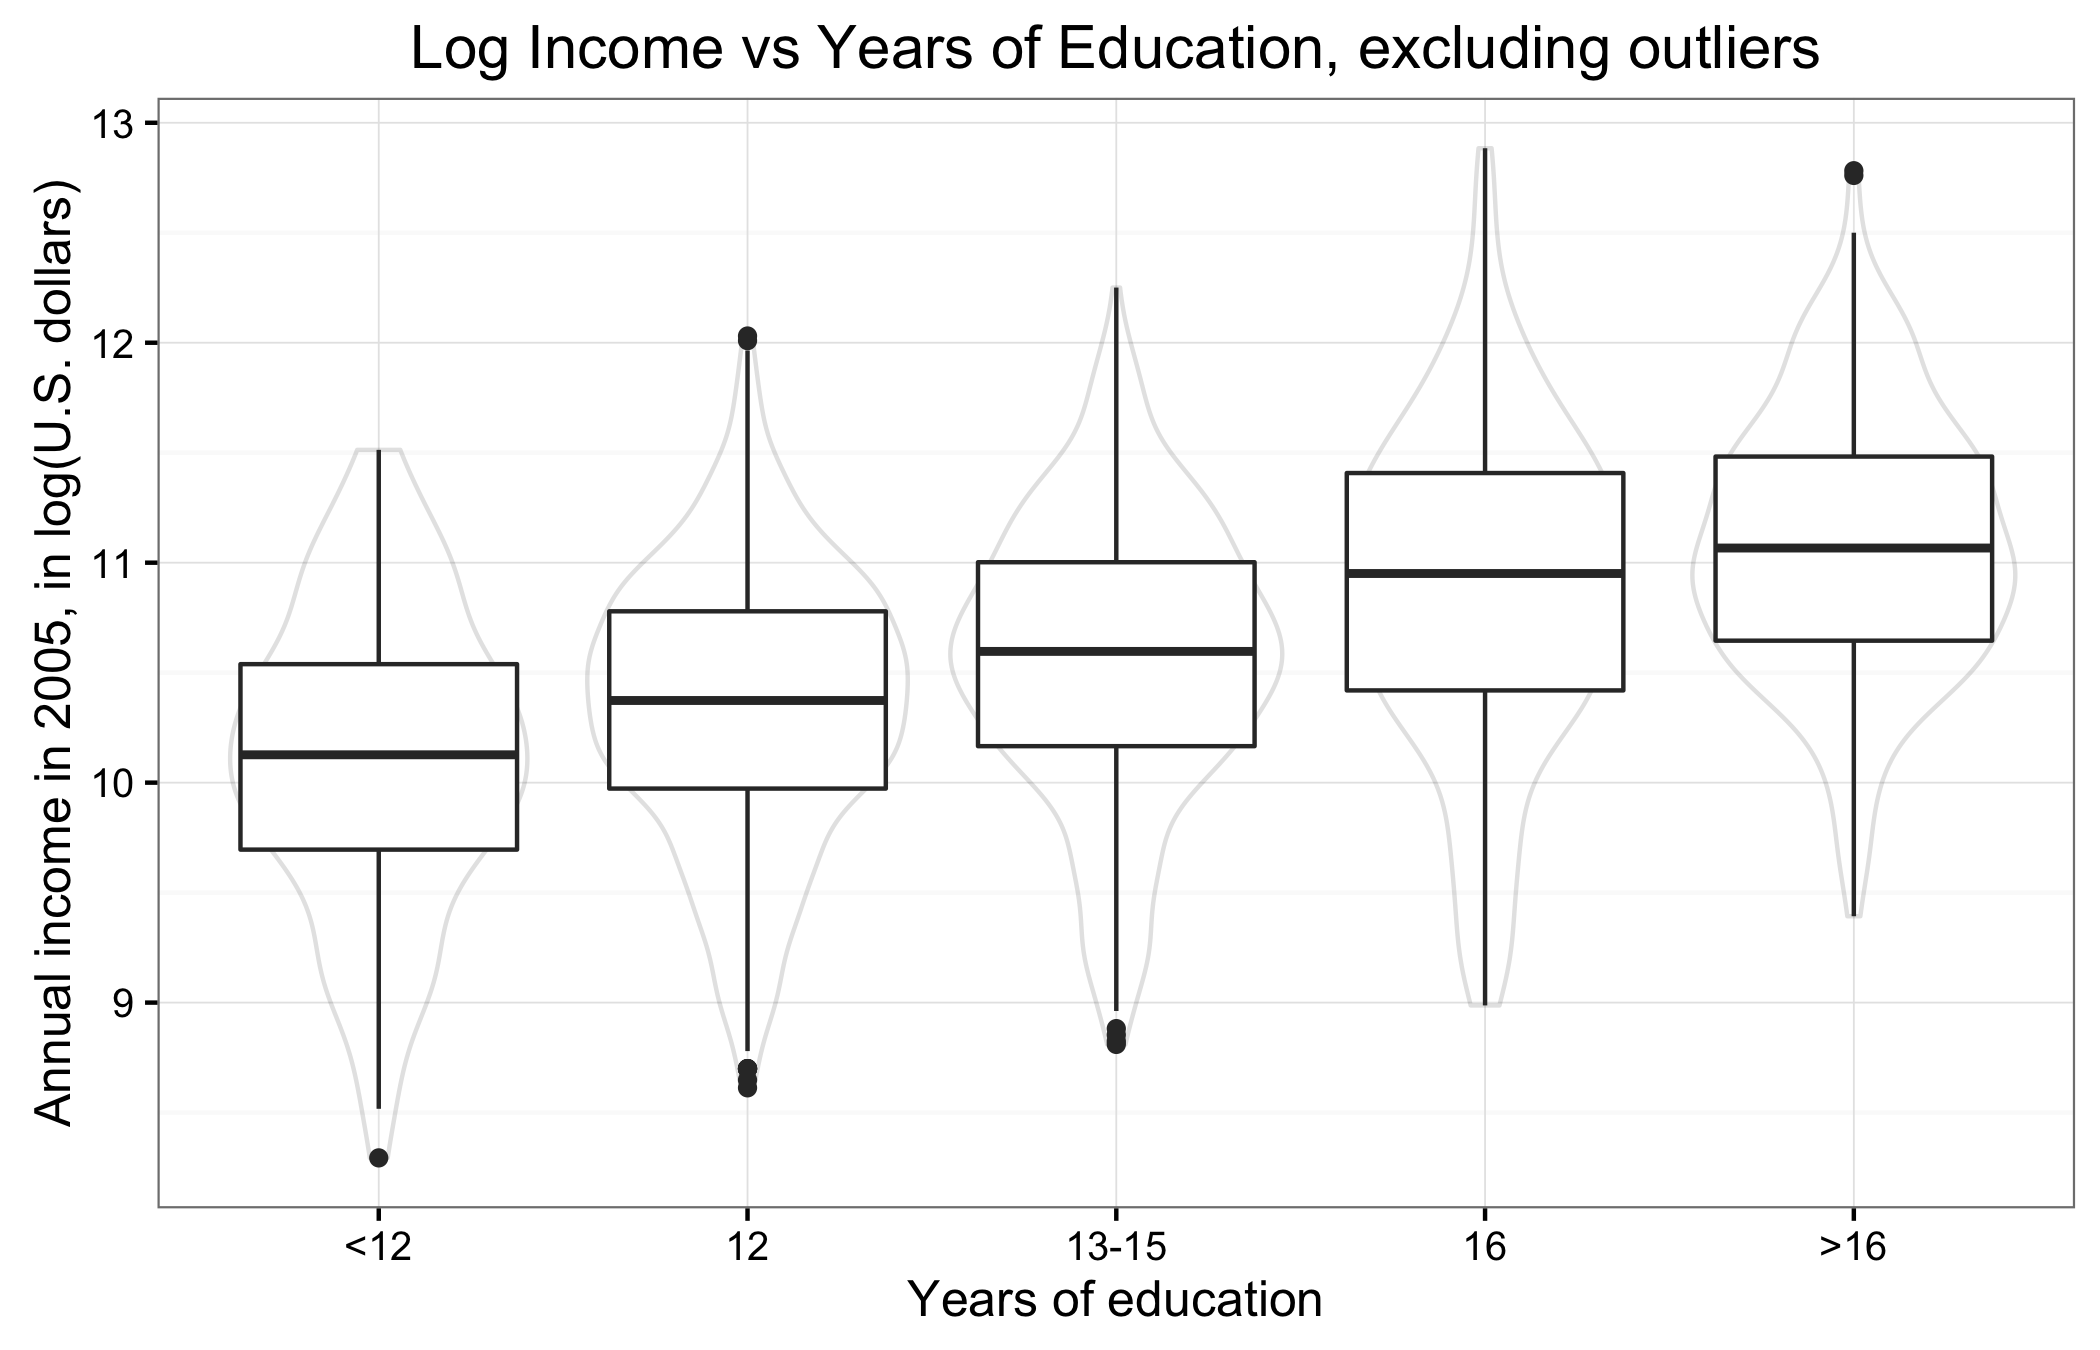
\includegraphics[width=5in]{2c.png}
%	%\caption{}
%	%\label{fig:figName}
%\end{figure}


\end{parts}



\titledquestion{question name 2}

\begin{parts}

\part \lipsum[3-5]


\end{parts}





\end{questions}

\listoftodos

\end{document}
